\documentclass[12pt,a4paper]{article}
\usepackage[utf8]{inputenc}
\usepackage[T1]{fontenc}
\usepackage{amsmath}
\usepackage{amsfonts}
\usepackage{amssymb}
\usepackage{lipsum}
\usepackage{textcomp}

\usepackage{makecell} % linebreak dans une cellule
\usepackage{multicol} % twocols localement
\usepackage{vwcol} % idem mais avec largeur variable
\usepackage{color, colortbl} % colorer les tableaux
\usepackage{enumitem} % utiliser des lettres pour énumérer
\usepackage{wrapfig} % insérer des images dans dutexte
\usepackage{dashundergaps} % transformer du texte en ________
\usepackage{MnSymbol,wasysym} % smileys
\usepackage{ifthen}
\usepackage{soul} % teste barré \st

% --- geometry ---
\usepackage{geometry}
\geometry{legalpaper, margin=2cm}
% ---

% --- xcolor ---
\usepackage{xcolor}
\definecolor{lightgray}{gray}{0.9}
% ---

% --- tcolorboxes ---
\usepackage[most]{tcolorbox}
\newtcolorbox{definition}[2][]{%
  attach boxed title to top left
               = {yshift=-8pt},
  colback      = white,
  colframe     = gray,
  fonttitle    = \bfseries,
  colbacktitle = gray,
  title        = #2,#1,
  enhanced,
}
% ---


\renewcommand{\baselinestretch}{1.15} % augmenter l'interligne

\dashundergapssetup{
	teacher-gap-format=underline,
	gap-widen
}



\author{Paul Clavier}
\title{Chapitre 2 - Les nombres décimaux}

\begin{document}

% --- Section & subsection renum ---
\renewcommand\thesection{\Roman{section}}
\renewcommand\thesubsection{\arabic{subsection}}
% ---

% --- Selection manuelle de la version ---
%\TeacherModeOn
% ---

% --- Selection automatique de la version ---
\ifdefined\isprof
	\TeacherModeOn
\fi

% ---



\begin{center}
	\fbox{\huge Chapitre 2 - Les nombres décimaux}
\end{center}

\section{Nombres entiers}

\begin{definition}{Différence entre chiffres et nombres}
0,1,2,3,4,5,6,7,8,9 sont les 10 \gap*{chiffres} qui permettent d'écrire tous les \gap*{nombres} (de même que les lettres de A à Z permettent d'écrire tous les mots).\\
\textbf{Exemples}:\\
1054 est un \gap*{nombre} de \gap*{4 chiffres}. 7 est un \gap*{nombre} d'un seul \gap*{chiffre}.
\end{definition}

\section{Lire et écrire un nombre entier}
La position des chiffres dans l'écriture du nombre permet de déterminer la quantité d'unités correspondante, la quantité de dizaines correspondantes, ….\\
\textbf{Exemples}: 45 se décompose en (4x10) + 5 ; 651 se décompose en \gap*{(6x100) + (5x10) + 1}\\
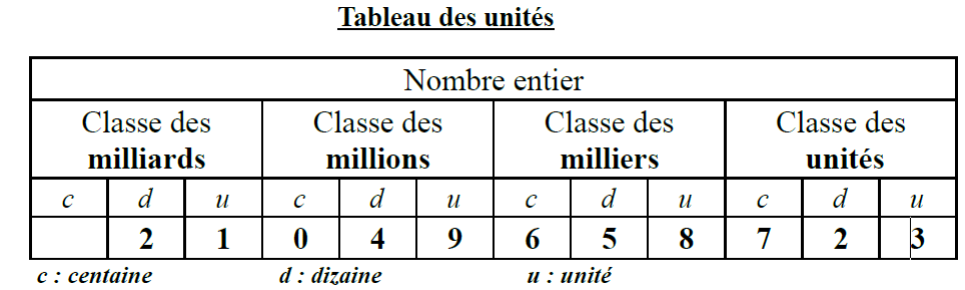
\includegraphics[scale=0.70]{img/tableau-unites.png} 
Pour lire facilement un nombre entier, on sépare son écriture en tranche de trois chiffres à partir de la droite :\\
Exemple : 21049658723 $\rightarrow$ 21 049 658 723
Ce nombre s'écrit en chiffres : \gap*{21 049 658 723}\\
Il s'écrit en toutes lettres :
\gap*{vingt-et-un milliards quarante-neuf millions six cent cinquante-huit mille sept cent vingt-trois}

Cas particuliers et règles d'orthographe:
\begin{itemize}
\item Les nombres composés s'écrivent avec des traits d'union. « 21 » s'écrit: vingt-et-un
\item Le nombre mille (1 000) est invariable (il ne prend jamais de « s »). « 2 000 » s'écrit deux mille
\item Les nombres vingt (20) et cent (100) ne prennent pas de « s » au pluriel lorsqu'ils sont suivis d'un autre nombre, sinon ils s'accordent:
\begin{itemize}
\item « 80 » s'écrit quatre-vingts
\item « 300 » s'écrit trois cents « 401 » s'écrit quatre cent un
\end{itemize}
\end{itemize}

\section{Les nombres décimaux}
\subsection{Écriture décimale}
Un nombre décimal se décompose en deux parties séparées d'une virgule:
\begin{itemize}
\item La partie entière
\item La partie décimale, qui comporte un nombre fini de chiffres non nuls
\end{itemize}

\begin{center}
\begin{tabular}{rcl}
1835 & , & 34 \\ 
\gap*{partie entière} &  & \gap*{partie décimale} \\ 
\end{tabular} 
\end{center}
4,33333.... n'est pas un nombre décimal car la partie décimale de ce nombre est infinie.\\
\begin{definition}{Remarque}
Un nombre entier est un nombre décimal dont la partie entière est nulle.
\end{definition}

\begin{definition}{Propriété}
On ne change pas un nombre décimal si on ajoute ou on enlève:
\begin{itemize}
\item des 0 avant la partie entière
\item des 0 après la partie décimale
\end{itemize}
On peut donc simplifier l'écriture d'un nombre en supprimant les 0 inutiles.
\end{definition}

\textbf{Exemples}: Rayer les 0 inutiles:
\begin{center}
\ifdefined\isprof
3,06\st{00} - 401,3\st{00} - 14\st{,0} - 13 400 - \st{0}27,08\st{0}
\else
3,0600 - 401,300 - 14,0 - 13 400 - 027,080
\fi
\end{center}
L'écriture sans zéro inutiles s'appelle l'écriture réduite.

\subsection{Rang des chiffres d'un nombre décimal}
\textbf{Attention: on place toujours le chiffre des unités en premier !}\\
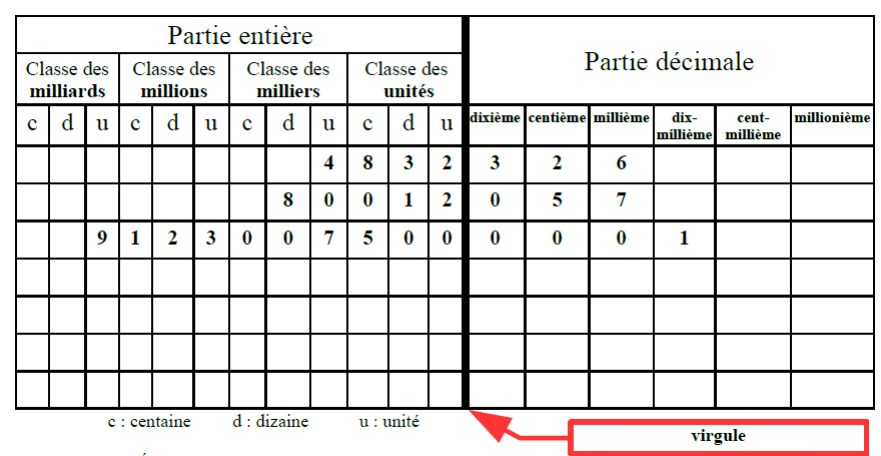
\includegraphics[scale=0.75]{img/tableau-unites-2.png} 

Les nombres décimaux peuvent aussi se décomposer. Par exemple:
\begin{center}
456,23 = (4 x 100) + (5x10) + (6x1) + (2x0,1) + (3x0 ,01)
\end{center}
\textbf{Exercice}:
\begin{enumerate}[label=\textbf{\alph*.}]
\item Écrire correctement les trois nombres placés dans le tableau\\
\gap*{4 832,326} - \gap*{80 012,057} - \gap*{9 123 007 500,000 1}
\item Placer dans le tableau 15 000,5 - 366 008,701 - 25 032 780,098
\item Placer dans le tableau le nombre 1 865,34
\begin{itemize}
\item Le chiffre des dizaines de 1 865,34 est \gap*{6\hbox{0000}}
\item Le nombre de dizaines de 1 865,34 est \gap*{186\hbox{00}}
\item Le chiffre des dixièmes de 1 865,34 est \gap*{3\hbox{0000}}
\item Le nombre de dixièmes de 1 865,34 est \gap*{18 653}
\end{itemize}
\end{enumerate}

\subsection{Différentes écritures d'un nombre décimal}

\begin{definition}{Définition}
Une \textbf{fraction décimale} est une fraction qui a pour dénominateur 10, 100, 1 000, ...\\
Elle représente un nombre décimal.
\end{definition}

\begin{definition}{Exemple}
\begin{center}
28,36
\end{center}
\begin{description}
\item[Écriture en lettres]: vingt-huit unités et trente-six centièmes
\item[Écriture décimale]: 28,36
\item[Partie entière]: 28
\item[Partie décimale]: 0,36
\item[Écriture décomposée]: $ (2\times 10) + (8\times 1) + (3\times 0,1) + (6\times 0,01) $
\item[Écriture en fraction décimale]: $\displaystyle\frac{2836}{100}$
\end{description}
\end{definition}

\textbf{Exercice}: Compléter le tableau suivant


\begin{tabular}{|c|c|c|c|c|@{}m{0cm}@{}}
\hline 
\thead{Écriture\\ décimale} & \thead{Partie\\ entière} & \thead{Partie\\ décimale} & Écriture décomposée & Fraction décimale \\ 
\hline 
192,384 & \gap*[b]{192} & \gap*[b]{0,384} & \thead{\gap*[b]{$ (1\times 100) + (9\times 10) + (2\times 1) $}\\ \gap*[b]{$+ (3\times 0,1) + (8\times 0,01) + (4\times 0,001) $}} & \gap*[b]{$\displaystyle\frac{192 384}{1000}$} & \thead{\\ \\ \\} \\ 
\hline 
\gap*[b]{17,981} & 17 & 0,981 & \thead{\gap*[b]{$ (1\times 10) + (7\times 1) $}\\ \gap*[b]{$+ (9\times 0,1) + (8\times 0,01) + (1\times 0,001) $}} & \gap*[b]{$\displaystyle\frac{17 981}{1000}$} & \thead{\\ \\ \\} \\ 
\hline
0,97 & \gap*[b]{0} & \gap*[b]{0,97} & \thead{\gap*[b]{$(0\times 1) $}\\ \gap*[b]{$+ (9\times 0,1) + (7\times 0,01) $}} & \gap*[b]{$\displaystyle\frac{97}{100}$} & \thead{\\ \\ \\} \\ 
\hline 
\gap*[b]{400,07} & \gap*[b]{400} & \gap*[b]{0,07} & \thead{$ (4\times 100) +  (7\times 0,01) $} & \gap*[b]{$\displaystyle\frac{40007}{100}$} & \thead{\\ \\ \\} \\ 
\hline 
\gap*[b]{31} & 31 & 0 & \thead{\gap*[b]{$ (3\times 10) + (1\times 1) $}} & \gap*[b]{$\displaystyle\frac{31}{1}$} & \thead{\\ \\ \\} \\ 
\hline 
\gap*[b]{1,84} & \gap*[b]{1} & \gap*[b]{0,80} & \gap*[b]{$ (1\times 1) + (8\times 0,1) + (4\times 0,01)$} & $\displaystyle\frac{184}{100}$ & \thead{\\ \\ \\} \\ 
\hline 
\gap*[b]{0,0504} & \gap*[b]{0} & \gap*[b]{0,0504} & \gap*[b]{$ (5\times 0,01) + (4\times 0,0001)$} & $\displaystyle\frac{504}{10 000}$ & \thead{\\ \\ \\} \\ 
\hline 
\end{tabular} 

\end{document}